\label{chap:array_write_process}
This chapter provides the reader with an overview of the formatting of data required to drive an IRLED array, and hardware specific details of the underlying array write process in order to facilitate an understanding of the context in which PDP is implemented, as well as, highlight some of the challenges with high speed operation. Firstly, it discusses the interleaved write process required to directly drive LEDs on an LED IRSP. Then, it discusses the data re-ordering done to optimize the write process. Protocol level details of how external data is received are discussed in Chapter~\ref{chap:display_protocols}.


\section{Array Interleaved Write Process}
    \label{sec:array_Interleaved_write_process}
    Although all current IRSP arrays utilize some display protocol technology that is decoded pixel by pixel in order to drive an array's actual pixels, arrays may utilize different internal drawing mechanisms for driving pixels. This section discusses the details of those mechanisms within the TCSA, NSLEDS, and HDILED arrays for conceptual purposes, and while the details may differ for other arrays, the overall raster write process is generalizable in the sense that not all pixels will be driven at once but some subset. Even arrays which operate in a snapshot mode where all pixels turn on at the same time will charge subsets of pixels over some time frame and enable the pixels only once all are charged. The write order and number of pixels driven at the same time would be array dependent though.

    %FIXME: add proper citation for Tianne paper when published
    The TCSA, NSLEDS, and HDILED arrays are organized into four quadrants as shown in Figure~\ref{fig:tcsa_nsleds_hdiled_quads}. Each quadrant is organized into a given number of pixels with TCSA housing 256 by 256, NSLEDS housing 512 by 512, and HDILED housing 1024 by 1024 per quadrant. There are number of input signals necessary to drive an array. These are {\em a 4 bit quadrant write enable}, {\em X address}, {\em Y address}, {\em LOAD bit}, {\em 16 Strong/Weak drive strength bit}, {\em array reset bit}, and {\em analog signaling lines which charges the pixels being addressed}. The quadrant write enable, X address, Y address, and LOAD signals are all utilized for addressing the array.

    \begin{figure}
        \centering
        %includegraphs[trim=L B R T]
        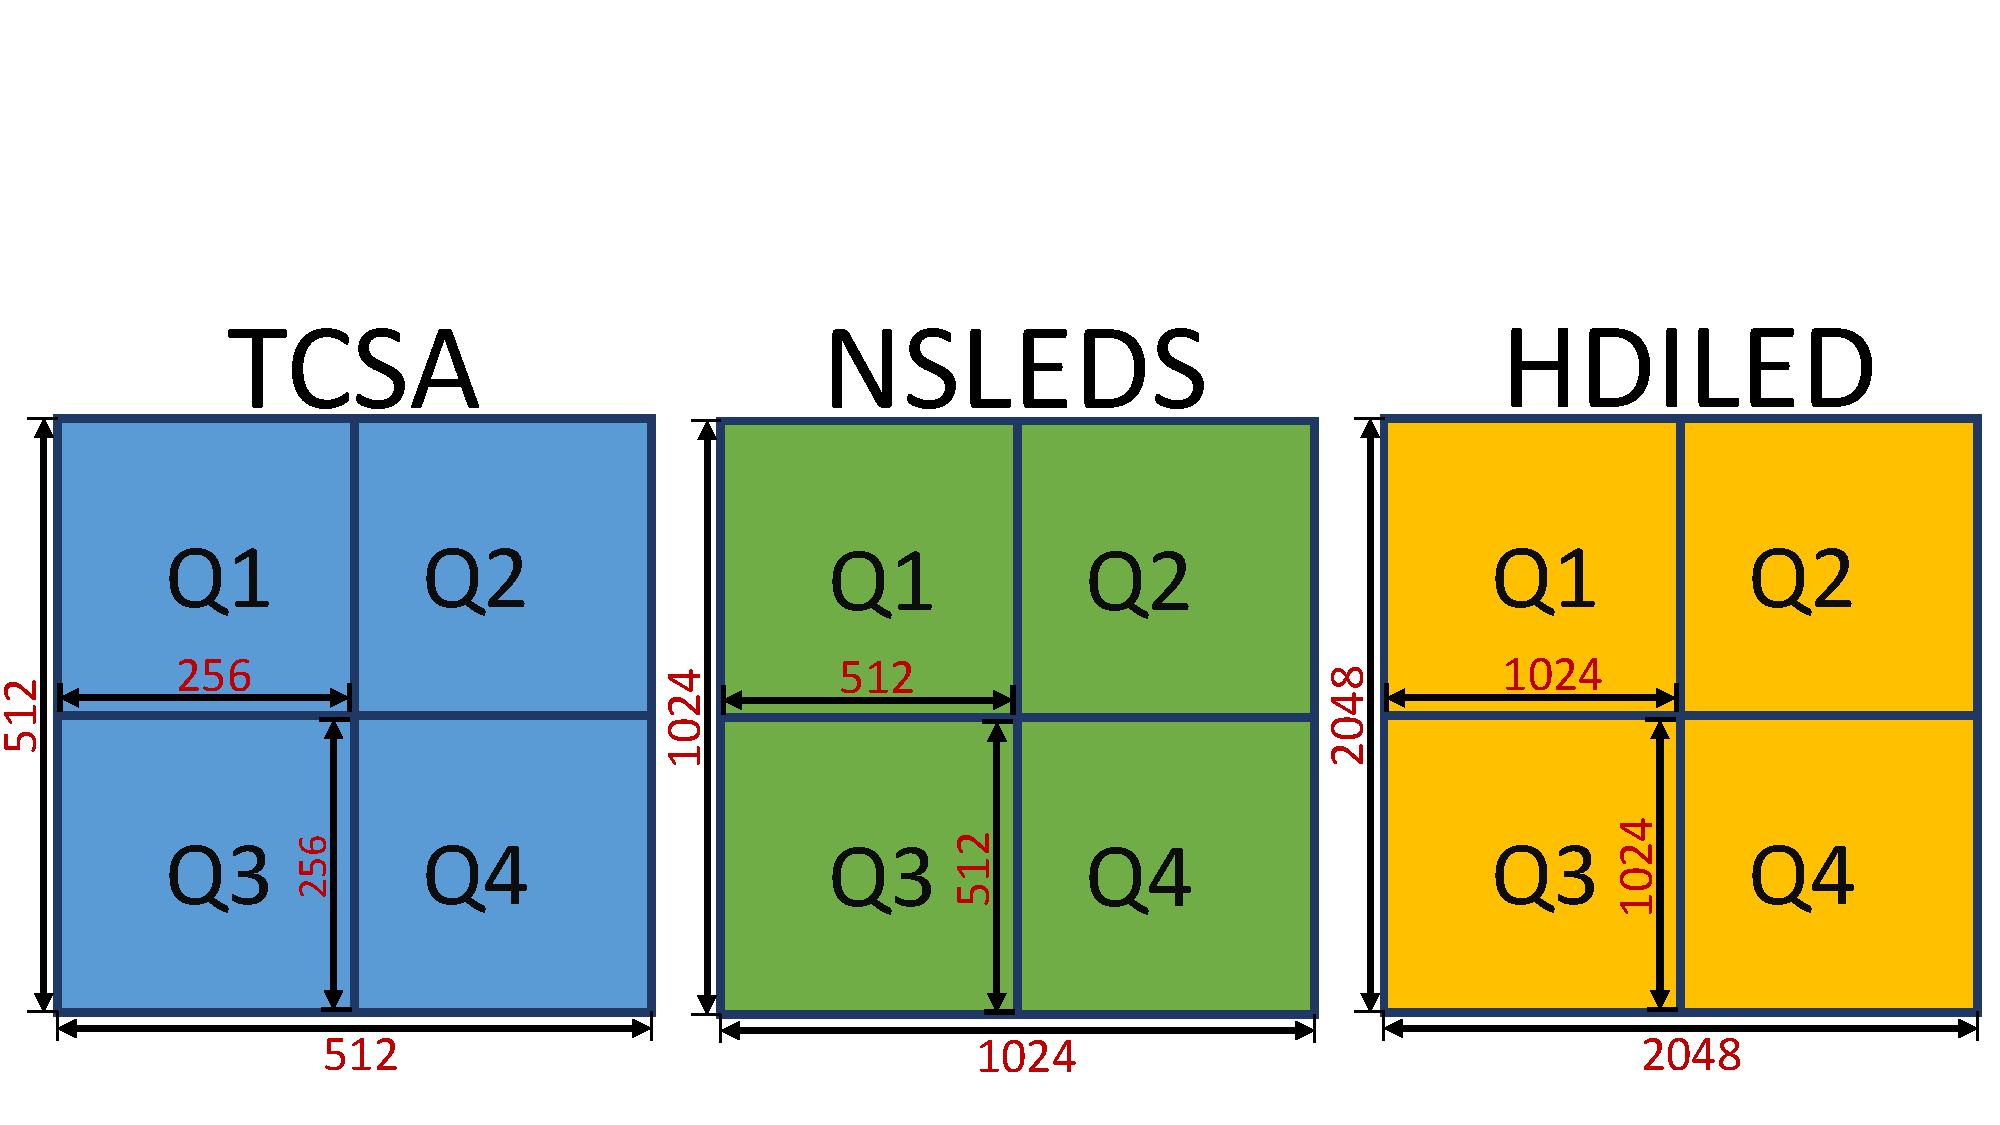
\includegraphics[width=1.0\textwidth]{fig/tcsa_nsleds_hdiled_quads.pdf}
        \caption[TCSA, NSLEDS, and HDILED Array Quadrant Layouts]{TCSA, NSLEDS, and HDILED Array Quadrant Layouts\textsuperscript{a}}
        \vspace{-8px}
        \footnotesize\textsuperscript{a} Not drawn to scale
        \label{fig:tcsa_nsleds_hdiled_quads}
    \end{figure}

    The quadrant write enable selects which quadrant to drive. It is worth noting that each quadrant has separate internal signaling which allows for each quadrant to operate independently in parallel when mounted in a package that provides independent external signals. However, to date most of the fabricated IRLED arrays are mounted in packages that allows for only one quadrant to be drawn at a time\footnote{Currently, only HDILED has been tested in the type of setup\cite{lassiter1, LassiterEtAl2019_1, LassiterEtAl2019_2, lassiter3} due to it having the largest resolution per quadrant.}. In a setup being driven in parallel, multiple CSEs are utilized. In a two CSE setup, half of the quadrant bits would be controlled by one CSE and half by another. In a four CSE setup, a single quadrant would be controlled by a single CSE. Irrespective of the number of CSEs used to a drive an array, the internal RIIC signal lines would be driven in precisely the same manner within each quadrant with the only change being that they operate asynchronously with respect to the others.

    The X address, Y address, and LOAD are used to select which pixel or group of pixels to write within a quadrant depending on the mode of operation. Though these lines are effectively shared by quadrants in a single CSE Setup, within the RIIC architecture they can be driven independently for each quadrant. Internally, each array can write up to 32 pixels (or channels) of data at a given time. The mode of operation dictates whether 2, 4, 8, 16, or 32 channels are used. The number of address bits utilized depends on the mode of operation. The amount of address bits differs by array due to the differences in sizes. NSLEDS utilizes 7 bits for the X address and 7 bits for the Y address, yielding a total of 256 by 256 addresses per quadrant. The LOAD bit is used to select between even and odd rows, yielding an effective address space of 256 by 512 per quadrant. Because the smallest mode of operation writes 2 pixels at a time, this is sufficient to fully address the array. Similarly, HDILED utilizes 8 bits for the X address and 8 bits for the Y address, yielding a total of 512 by 512 addresses per quadrant. Again, as with NSLEDS, the LOAD bit is used to select between even and odd rows, yielding an effective address space of 512 by 1024 per quadrant. This is again sufficient to completely address the array since it also can at a minimize write 2 pixels at a time.

    Structurally, NSLEDS and HDILED are layed out as super pixel as shown in Figure~\ref{fig:nsleds_hdiled_array_superpixel_layout}. Each super pixel is made up of a grid of 4 pixels spanning two rows and columns. These are layed out across the array in a grid structure with NSLEDS consisting of 256 by 256 super pixels, and HDILED consisting of 512 by 512 super pixels. This image also highlights two points discussed above, the LOAD line selects between the top two pixels (even rows) and bottom two pixels (odd rows) of each super pixel in the quadrant, and the two selected pixels are both written at the same time. Additionally, these share a drive strength as noted in the diagram. This is controlled using the Strong/Weak drive strength bits which dictate whether to provide a strong or weaker light emission for the given pair of pixels.

    \begin{figure}
        \centering
        %includegraphs[trim=L B R T]
        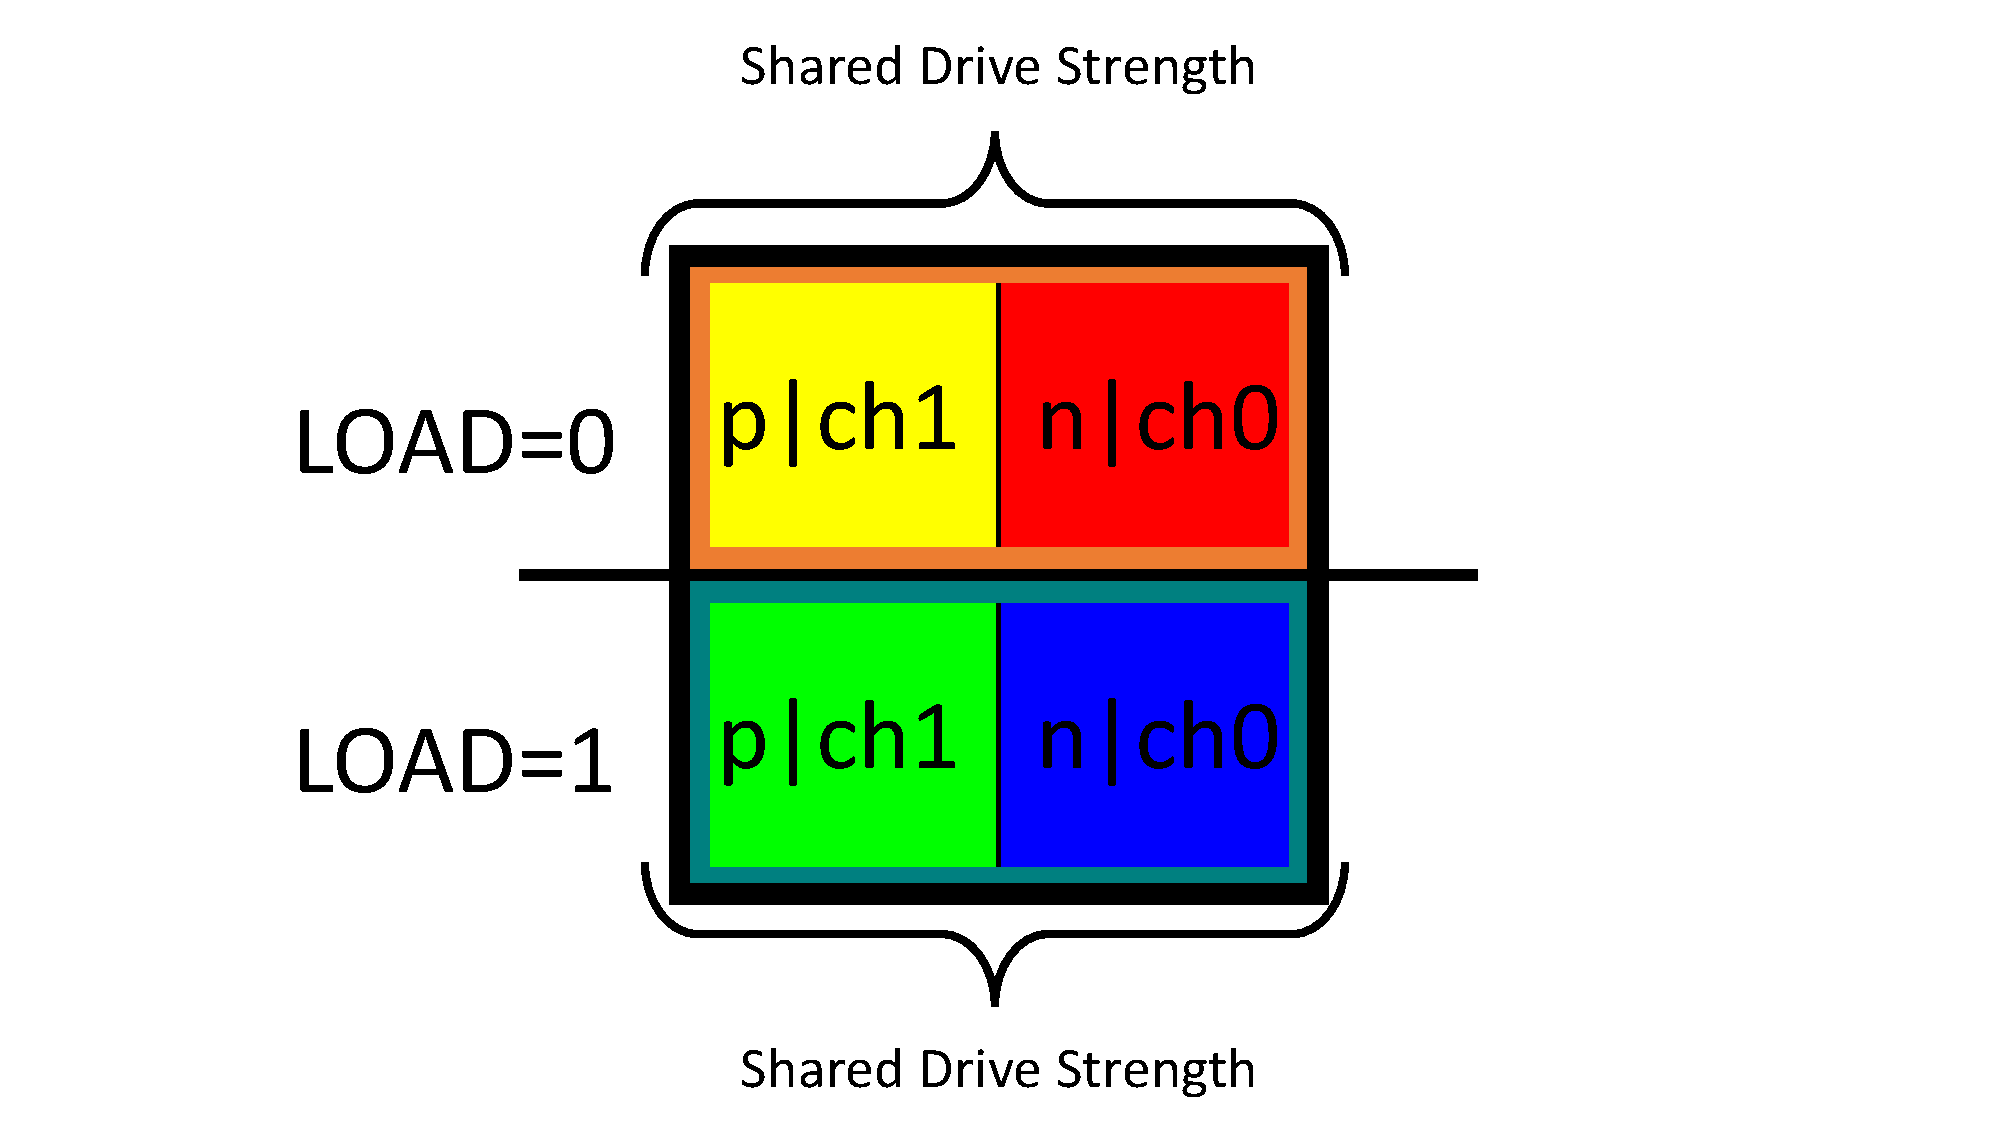
\includegraphics[width=0.70\textwidth]{fig/superpixel_layout.pdf}
        \caption{NSLEDS/HDILED Array Super Pixel Layout}
        \label{fig:nsleds_hdiled_array_superpixel_layout}
    \end{figure}

    The 32 analog signaling lines control the emission intensity of driven pixels. These 32 channels are controlled by digital to analog converters within the CSE that are driven by the firmware. Internally, a CSE has 8 DAC cards with 2 DAC integrated circuits per card, with each DAC circuit consisting of 2 DAC channels as discussed in Chapter~\ref{sec:close_support_electronics}. Each channel is used to drive a single pixel, giving the ability to drive 32 pixels at once or some subset as mentioned previously.

    In practice, it is perferable to utilize all channels at once because this allows for more pixels to be driven in a shorter amount of time. Figure~\ref{fig:nsleds_hdiled_array_interleaved_pixel_mapping_per_write} shows the pixel mapping per write for 32 physical pixels on an array. 2 by 32 columns of pixels are shown segmented into super pixels. The Y address denotes the 16 super pixels that are selected per address. If Y is incremented by 1 then the next 16 rows of super pixels would be selected. X address (not shown) simply selects the next two columns of super pixels. DAC Card denotes which DAC card drives the given super pixel. L denotes which value of LOAD will select which columns within super pixels. When LOAD is low as shown in the middle segment, the top super pixels are selected as indicated in cyan. When LOAD is high as shown in the right segment, the bottom super pixels are selected.

    \begin{figure}
        \centering
        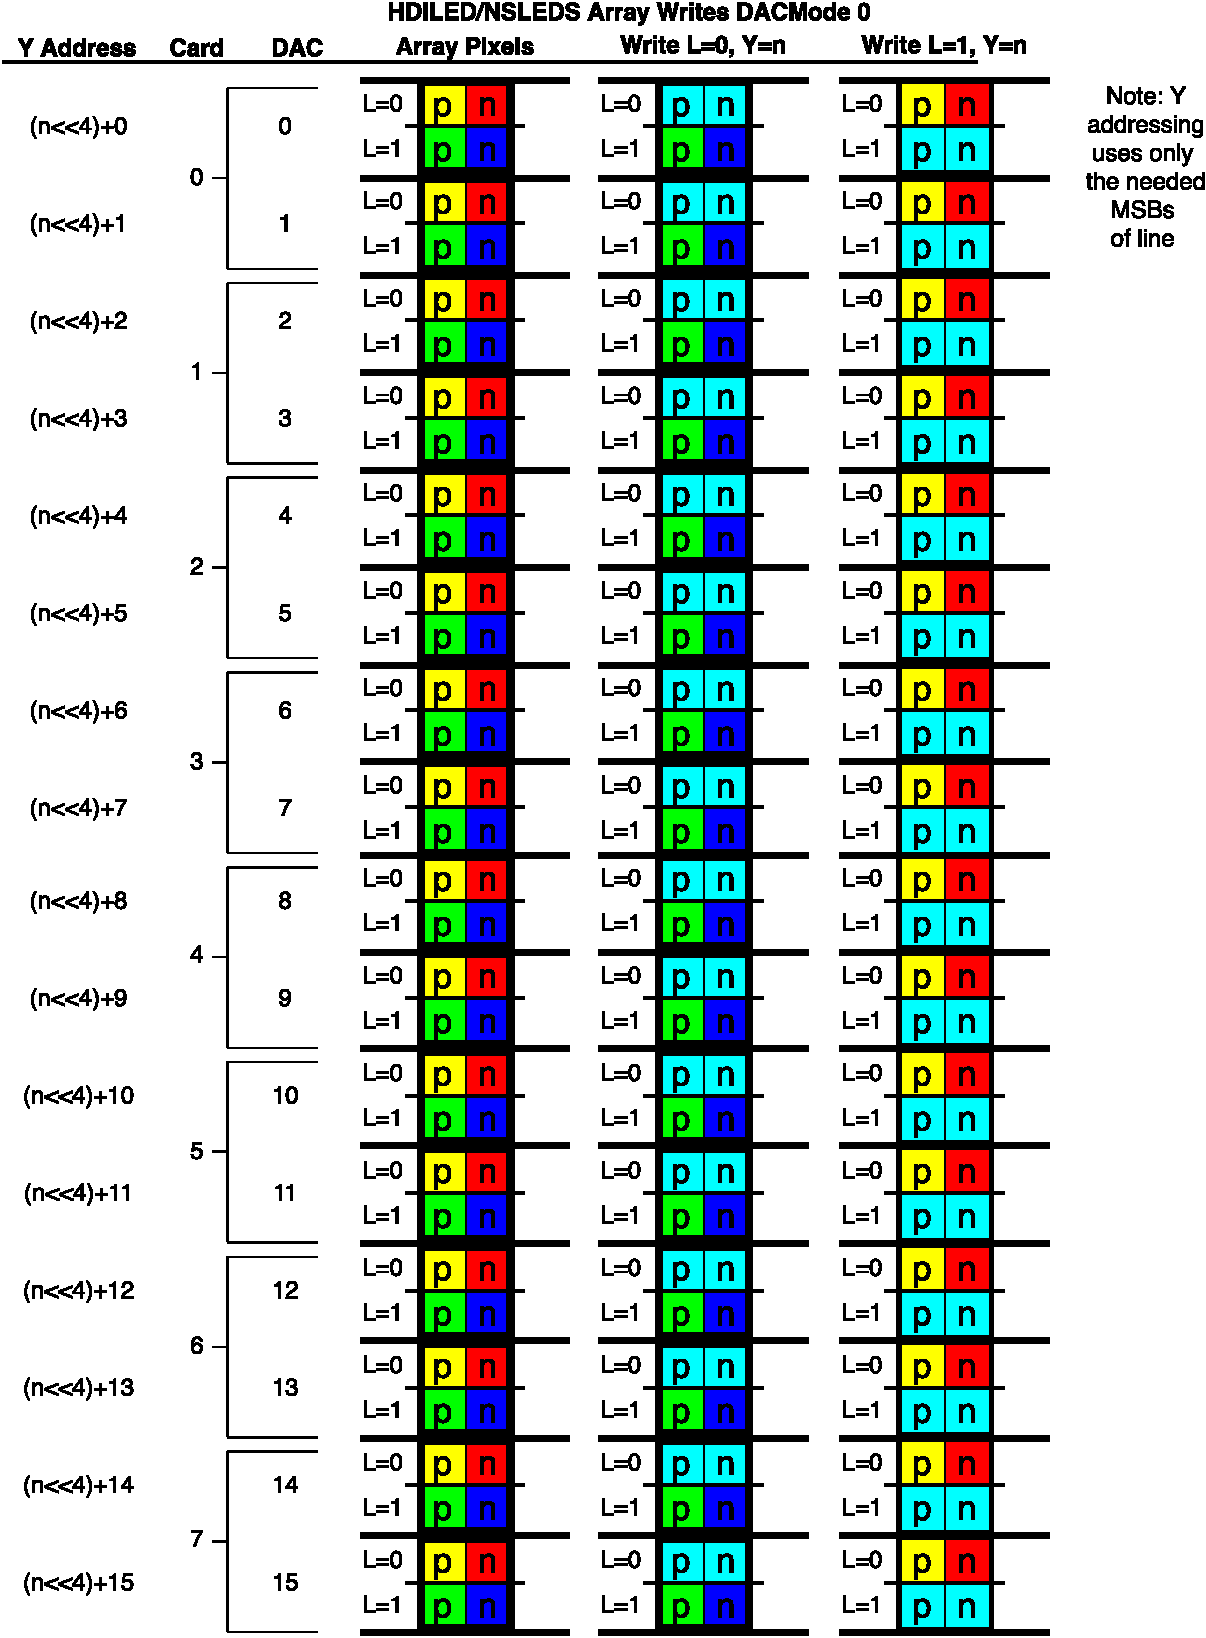
\includegraphics[width=0.95\textwidth]{fig/nsleds_hdiled_array_writing.pdf}
        \caption{NSLEDS/HDILED Array Interleaved Pixel Mapping Per Write}
        \label{fig:nsleds_hdiled_array_interleaved_pixel_mapping_per_write}
    \end{figure}

    The overall writing process for writing 64 pixels is a two step process. First, 32 values for the even rows are loaded in and written to the array, followed by 32 values from the odd rows being loaded and written to the array. At a data level, it is ideal to interleave the data such that it is avaliable at the optimal time in order to reduce latency and buffering requirements within the firmware. This is discussed in detail in Chapter~\ref{chap:pdp_protocol}.

    Writing additional segments of pixels largely means buffering more data and repeating the same write process while asserting the correct address lines. Given that the arrays have no inherit hardware required write order other than what has been discussed above, the exact order of writing independent segments of 32 pixels can change depending on a number of factors. In a single CSE Setup, under most circumstances, the data for the top quadrants is carried by a single HDMI input going into a CSE, and the data for the bottom quadrants carried by the other HDMI input\footnote{When utilizing PDP for driving an array the location of where data is to be written on an array is agnostic to the HDMI input the data is carried on.}. In this case, the CSE firmware will swap between writing segments of 32 or 64 pixels to the top and bottom halves of an array. The former if it is desirable to write a minimal amount of data before servicing data from another input, the latter if it is desirable to complete an entire chunk of pixels. In a two CSE Setup, data over the hdmi links data could be segmented either horizontally or vertically meaning that each HDMI link would carry an entire quadrants data. In a four CSE setup, each link would carry half a quadrants data. As the reader may imagine, the order of writes could be configured in many different ways under these scenerios. Though it will not be discussed in detail within this thesis, it is worth noting for posterity that the order of writes on IRLED arrays does affect the thermal load on an array which has an effect on pixel brightness\cite{BarakhshanEtAl2017, LaVeigneSieglinger2012, norton2}; thus, controlling the order of writes can be an important factor to consider for designers and users of a system.

    %FIXME: Add details about delays into the RIIC and aligning signals maybe?
    %FIXME: slow channels
\section{Data ordering}
    Due to the interleaved write process described in Chapter~\ref{sec:array_Interleaved_write_process}, data sent to an array is reordered in a manner that simplifies firmware development and minimizes buffering requirements. Figure~\ref{fig:bit_packing} shows the data bitpacking utilized within the system. It's designed to map to the superpixel layout shown in Figure~\ref{fig:nsleds_hdiled_array_superpixel_layout}. Shown is a 24-bit pixel word which normally represents an RGB value in RGB color space within display protocols where 8 bits are reserved for each of the red, green, and blue channels. Below this is the mapping of each bit value for an NSLEDS or HDILED array. Where \textbf{S} indicates the drive strength of the super pixel, \textbf{L} indicates the value to drive the left side of the super superpixel at, and \textbf{R} indicates the value to drive the right side of the superpixel at. Only 11 bits are currently used to transmit data per pixel due to bit resolution limitations in the DAC and amplifier boards used within a CSE\footnote{Future CSEs may have higher bit resolutions resulting in the need for 16-bits per pixel to be transmitted. In this event bitpacking would not be used}.

    \begin{figure}
        \centering
        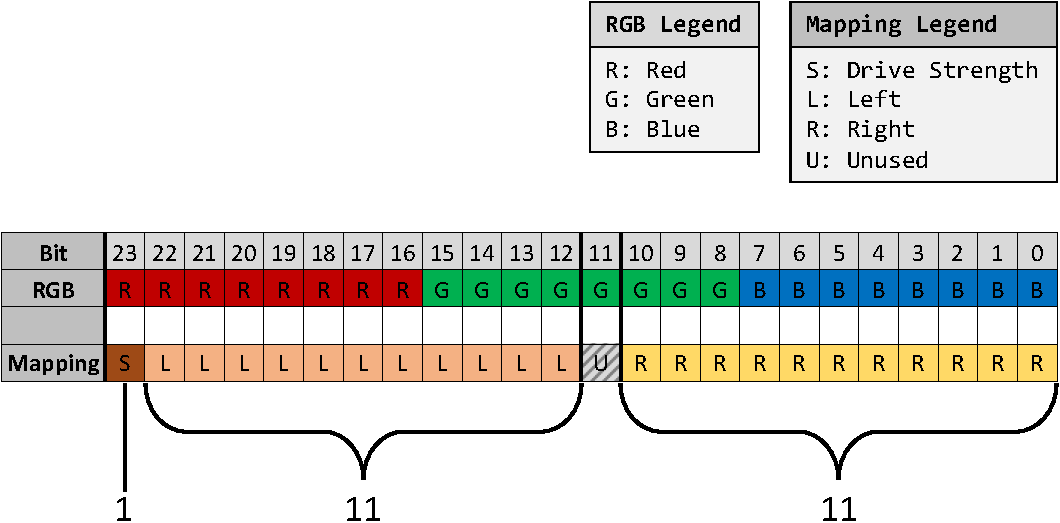
\includegraphics[width=1.0\textwidth]{fig/bit_packing.pdf}
        \caption{Bit-packing Format}
        \label{fig:bit_packing}
    \end{figure}

    Figure~\ref{fig:image_encoding} shows the input reordering needed to be done for data sent to a CSE. Each cable sends half of the data as noted in Chapter~\ref{sec:close_support_electronics}. The input example is segmented into top, middle, and bottom to indicate which part goes over which input and the different reordering steps. The portions denoted as \textbf{Top} are transmitted over CSE input 1. The portions denoted as \textbf{Bottom} are transmitted over CSE input 2. The portions marked \textbf{Middle} are split evenly over both inputs evenly. The first step of data reordering is to bitpack into 11-bit words as shown in Figure~\ref{fig:bit_packing}. Next, even/odd reordering is performed to reduce latency and buffering constraints as will be shown in more detail in subsequent figures. Finally, data is transposed before being sent to the array in order to accommodate the column write order of the array shown in Figure~\ref{fig:nsleds_hdiled_array_interleaved_pixel_mapping_per_write}. If data was not transposed in this manner, then multiple lines of data would need to be buffered in order to draw 32 pixels for a single write\footnote{Earlier pre-pdp firmware implementations required full image buffering before displaying a single pixel on an array resulting in an entire frame of latency}. It is worth noting that as mentioned in Chapter~\ref{sec:array_Interleaved_write_process}, different arrays could have different rasterization processess, and in that event the transformations described here would need to be changed to minimize buffering for those scenerios.


    \begin{figure}
        \centering
        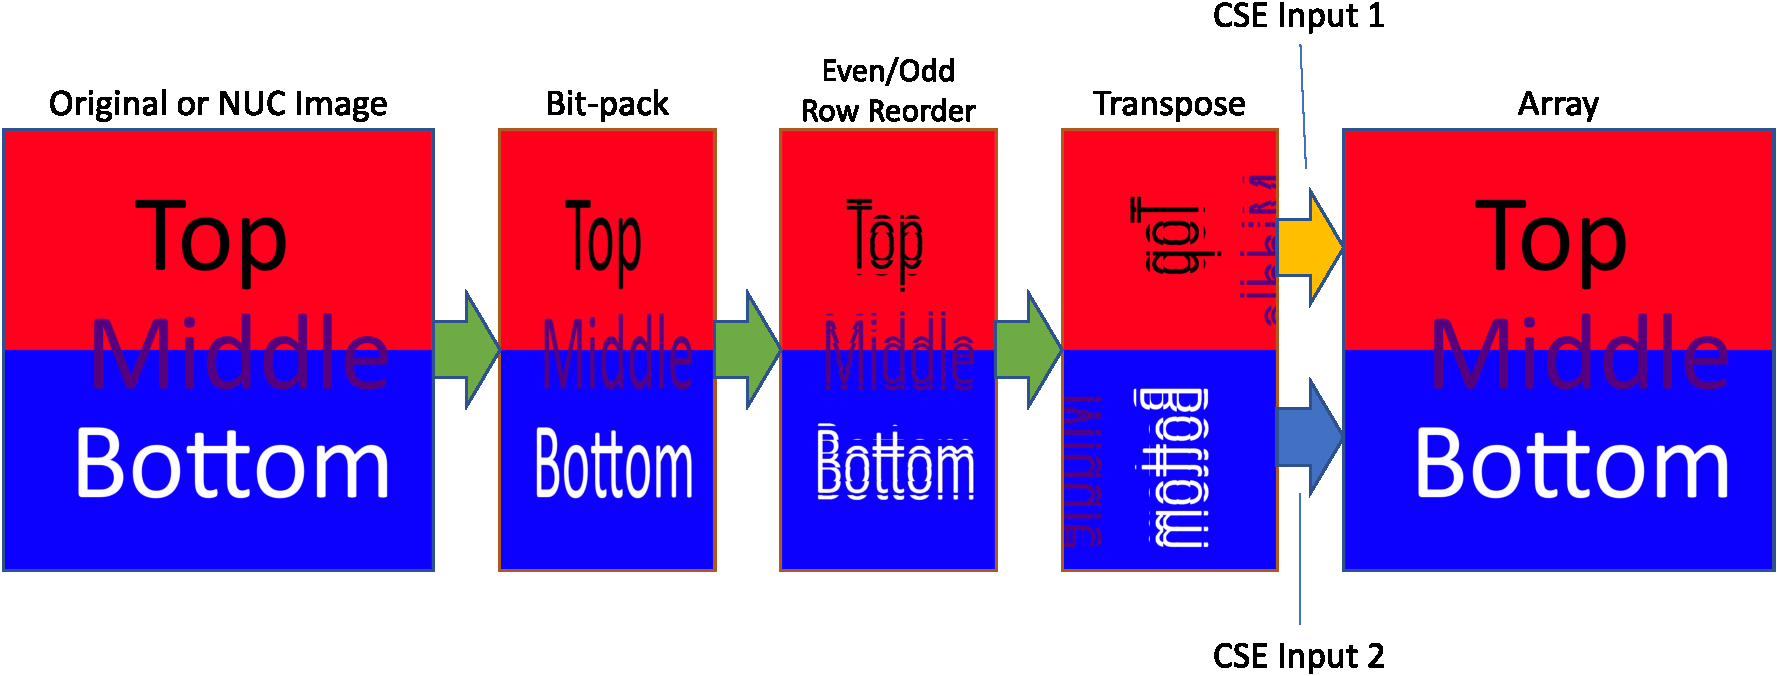
\includegraphics[width=1.0\textwidth]{fig/image_encoding.pdf}
        \caption{Image Encoding: Input Reordering}
        \label{fig:image_encoding}
    \end{figure}

    Figure~\ref{fig:image_encoding_quads} shows how the same image data maps to each quadrant on an array. Similarly, to the previous image the separation of top, middle, and bottom by input cable holds here. Additionally, shown is that quadrant one and two are transmitted over the first input and quadrant three and four over the second input. Note also, that the top-left of the image corresponds to quadrant one, the top-right of the image corresponds to quadrant two, the bottom-left of the image corresponds to quadrant three, and the bottom-right of the image corresponds to quadrant four. This relationship holds for all subsequent images. Figure~\ref{fig:image_encoding_colored} shows the same details in a colored chart.

    \begin{figure}
        \centering
        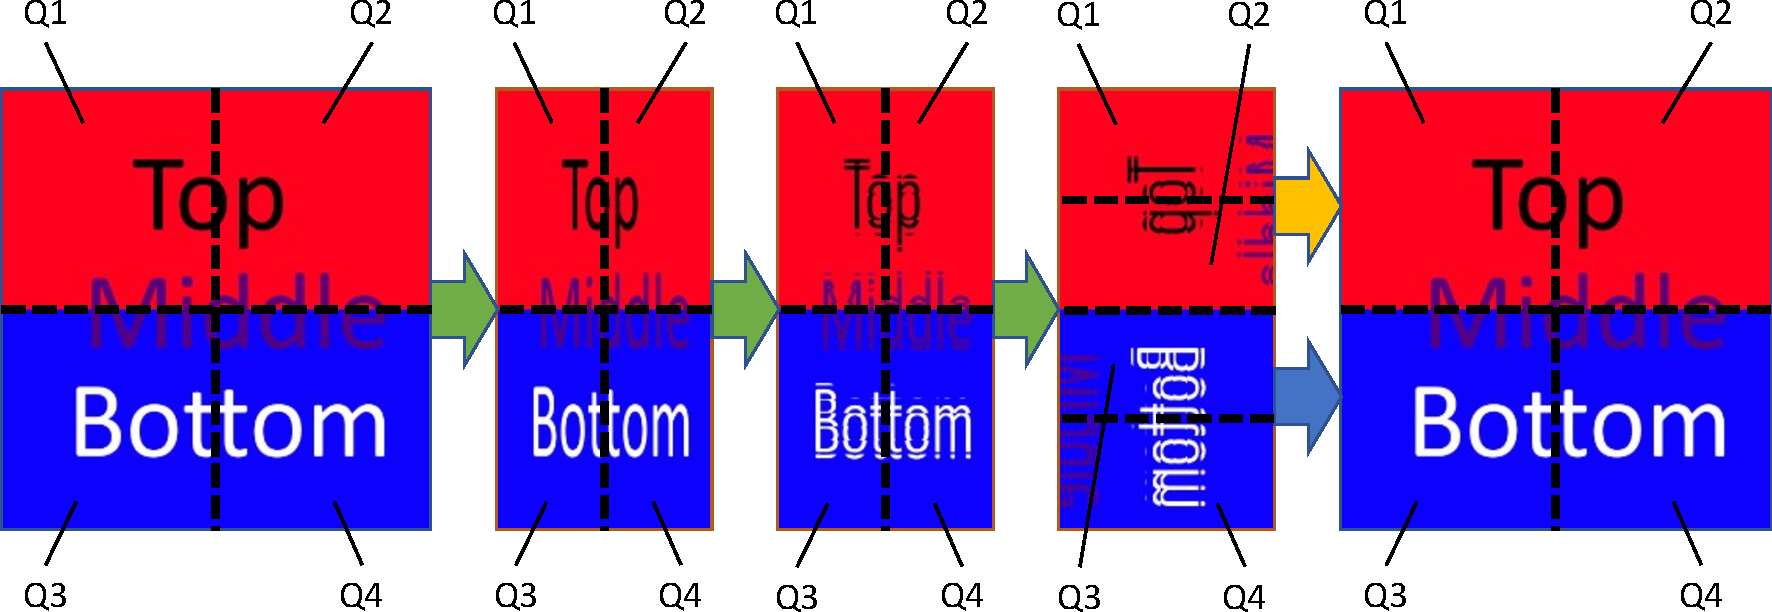
\includegraphics[width=1.0\textwidth]{fig/image_encoding_quads.pdf}
        \caption{Image Encoding: Quadrant Reordering}
        \label{fig:image_encoding_quads}
    \end{figure}

    \begin{figure}
        \centering
        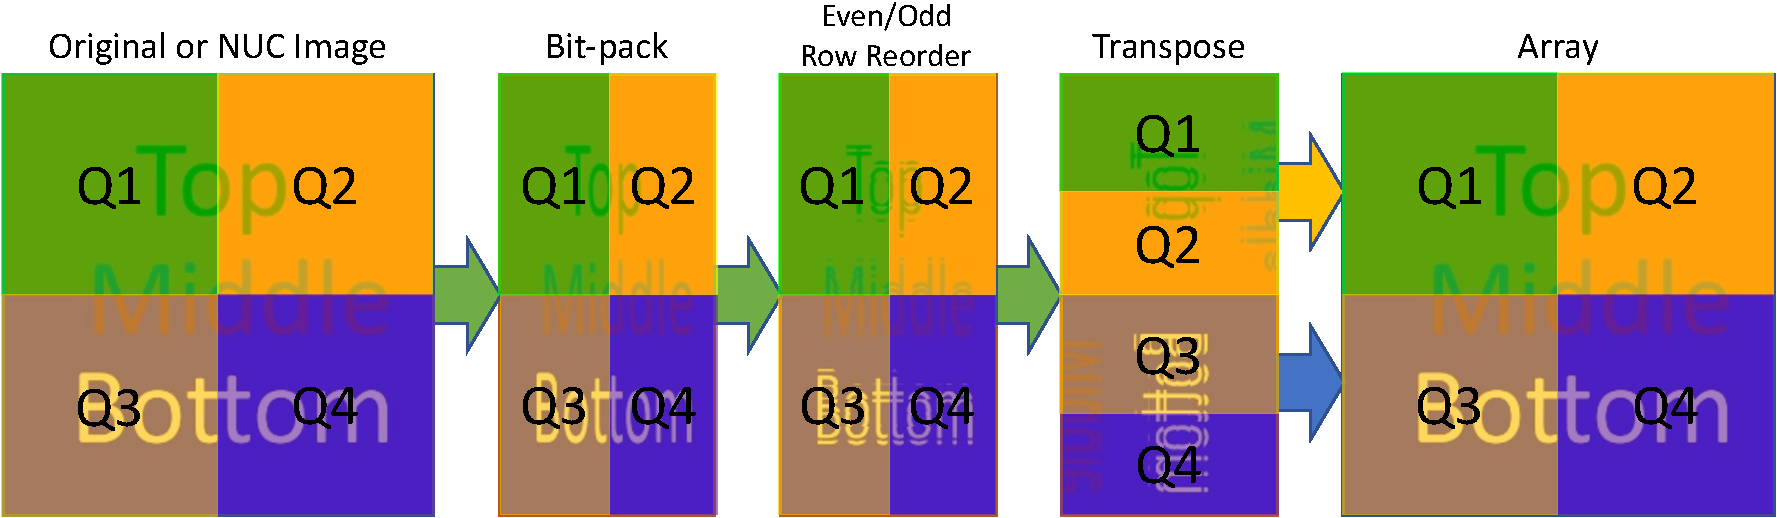
\includegraphics[width=1.0\textwidth]{fig/image_encoding_colored.pdf}
        \caption{Image Encoding: Quadrant Reordering with Color Overlay}
        \label{fig:image_encoding_colored}
    \end{figure}

    Figure~\ref{fig:image_encoding_bitback} shows the bit-packing process for a false color image in order to aid with understanding. The blown up sections show single columns of data and the cooresponding bitpacked version of the data where two columns of input with different colors of data per column are merged into a single column of 24-bit data with one color. This results in the example input image having two solid colors after bit-packing. In the actual implementation of bitpacking, real data is in the IR-spectrum and not averaged in this way, but clamped and scaled instead. While not required, generally IR data is normally 16-bits per pixel which corresponds to current higher class IR detectors having a dynamic range of 14 per pixel\cite{FLIR1, FLIR2, FLIR3}. Cheaper detectors may only have lower dynamic ranges resulting in a lower ability to differentiate light output.

    \begin{figure}
        \centering
        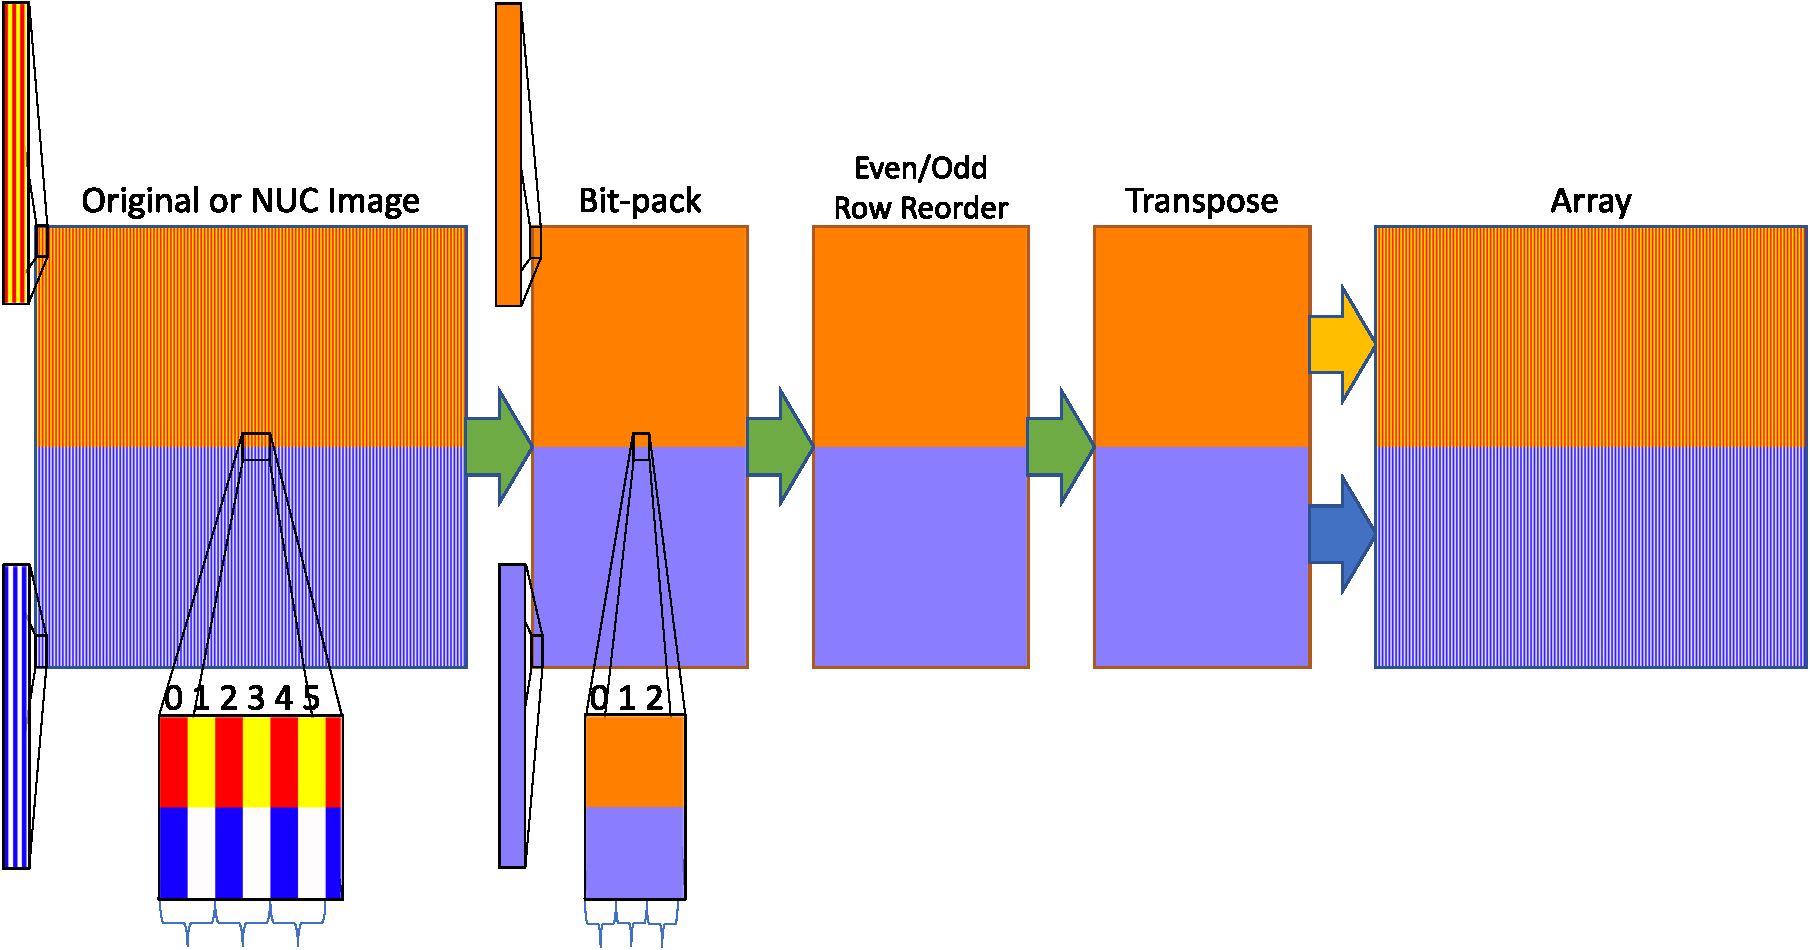
\includegraphics[width=1.0\textwidth]{fig/image_encoding_bitback.pdf}
        \caption{Image Encoding: Data Bitpack}
        \label{fig:image_encoding_bitback}
    \end{figure}

    Figure~\ref{fig:image_encoding_bitpack_reorder} shows a false color input image designed to highlight the data reordering applied to imagery. The blown up sections show 64 labeled rows of input data where the even rows are one color and the odd rows another for ever 32 rows. For every 32 rows, the even and odd rows are de-interlaced into 16 even rows of data follow by 16 odd rows of data. In the example input image this results in every 16 de-interlaced rows to have have a different color. This is due to the interleaved writing processing for individual 32 pixel writes discussed in Chapter~\ref{sec:array_Interleaved_write_process}. Reordering data in this manner allows for only 16 pixels of data (or 32 in terms of bitpacking) to be buffered per write. Without the is reordering, double the amount of pixels would need to be buffered per array write increasing both latency and implementation complexity.

    \begin{figure}[H]
        \centering
        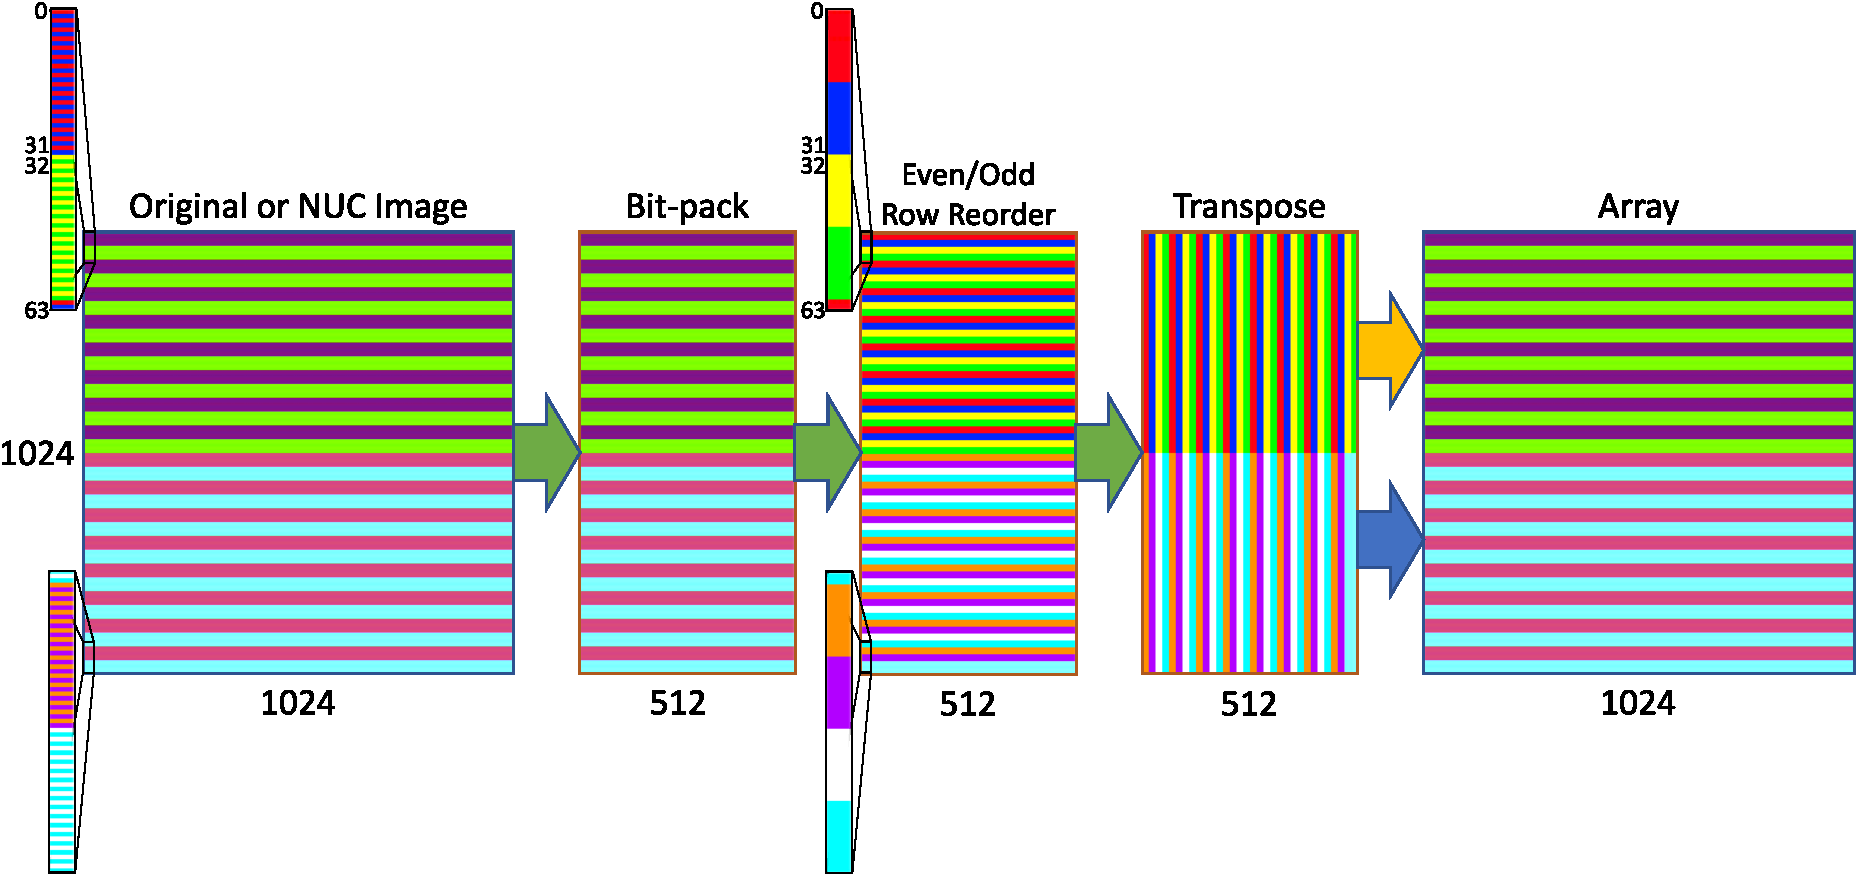
\includegraphics[width=1.0\textwidth]{fig/image_encoding_reorder.pdf}
        \caption{Image Encoding: Data Reorder}
        \label{fig:image_encoding_bitpack_reorder}
    \end{figure}

    Figures~\ref{fig:image_encoding_color_example1},~\ref{fig:image_encoding_color_example2},~and~\ref{fig:image_encoding_color_example3} show some examples of what false colored images would look like if processed by the reordering kernels in order to give the reader a better understanding of how different types of data would look when during the intermediate processes. Note the charateristic jagged pattern due to even/odd row reordering present in each image.

    \begin{figure}[H]
        \centering
        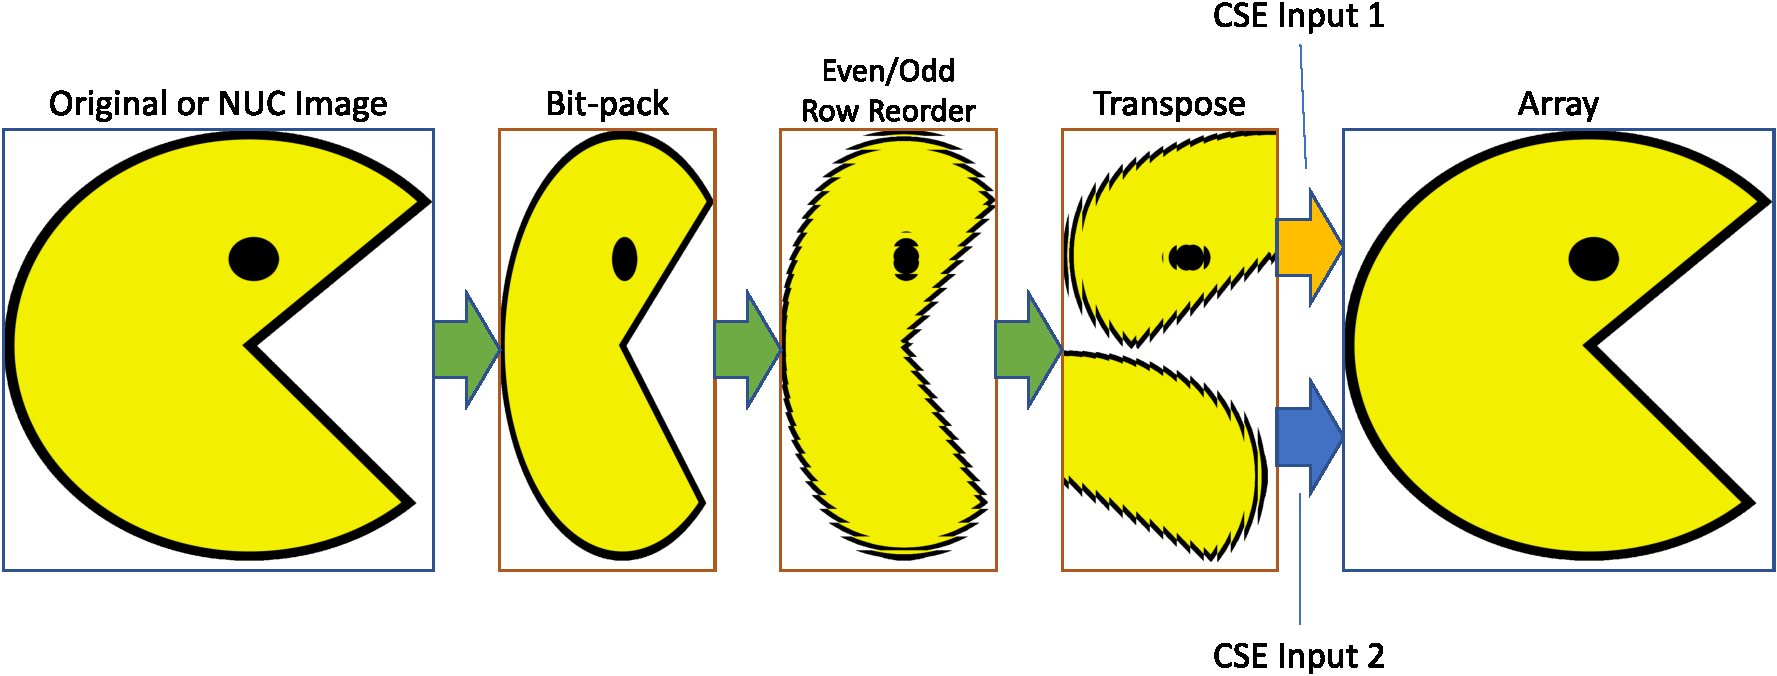
\includegraphics[trim=0 40pt 0 40pt,width=0.90\textwidth]{fig/image_encoding_pac.pdf}
        \caption{Image Encoding: Color Example 1}
        \label{fig:image_encoding_color_example1}
    \end{figure}

    \begin{figure}[H]
        \centering
        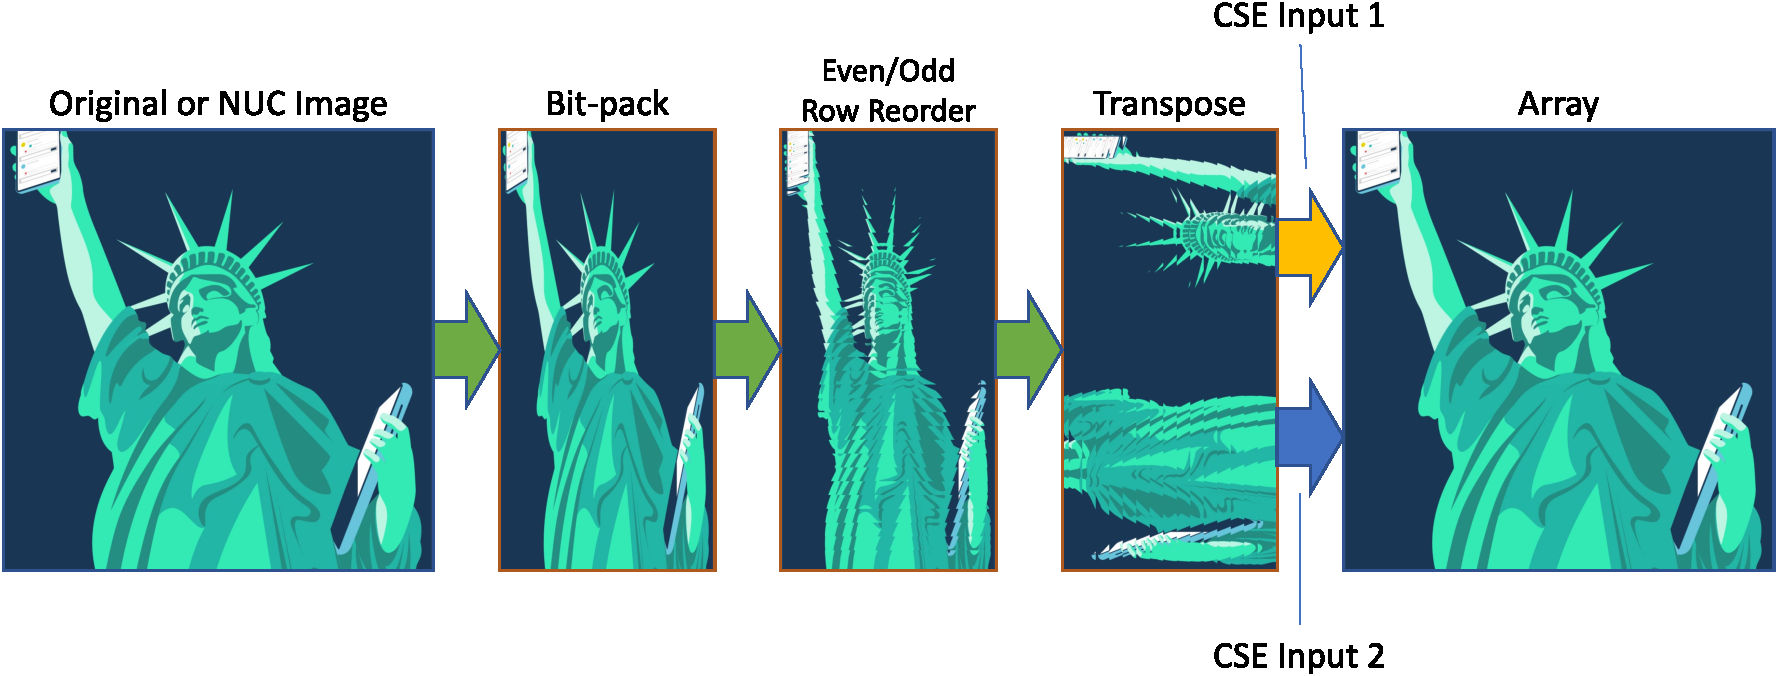
\includegraphics[trim=0 40pt 0 40pt,width=0.90\textwidth]{fig/image_encoding_liberty.pdf}
        \caption{Image Encoding: Color Example 2}
        \label{fig:image_encoding_color_example2}
    \end{figure}

    \begin{figure}[H]
        \centering
        %includegraphs[trim=L B R T]
        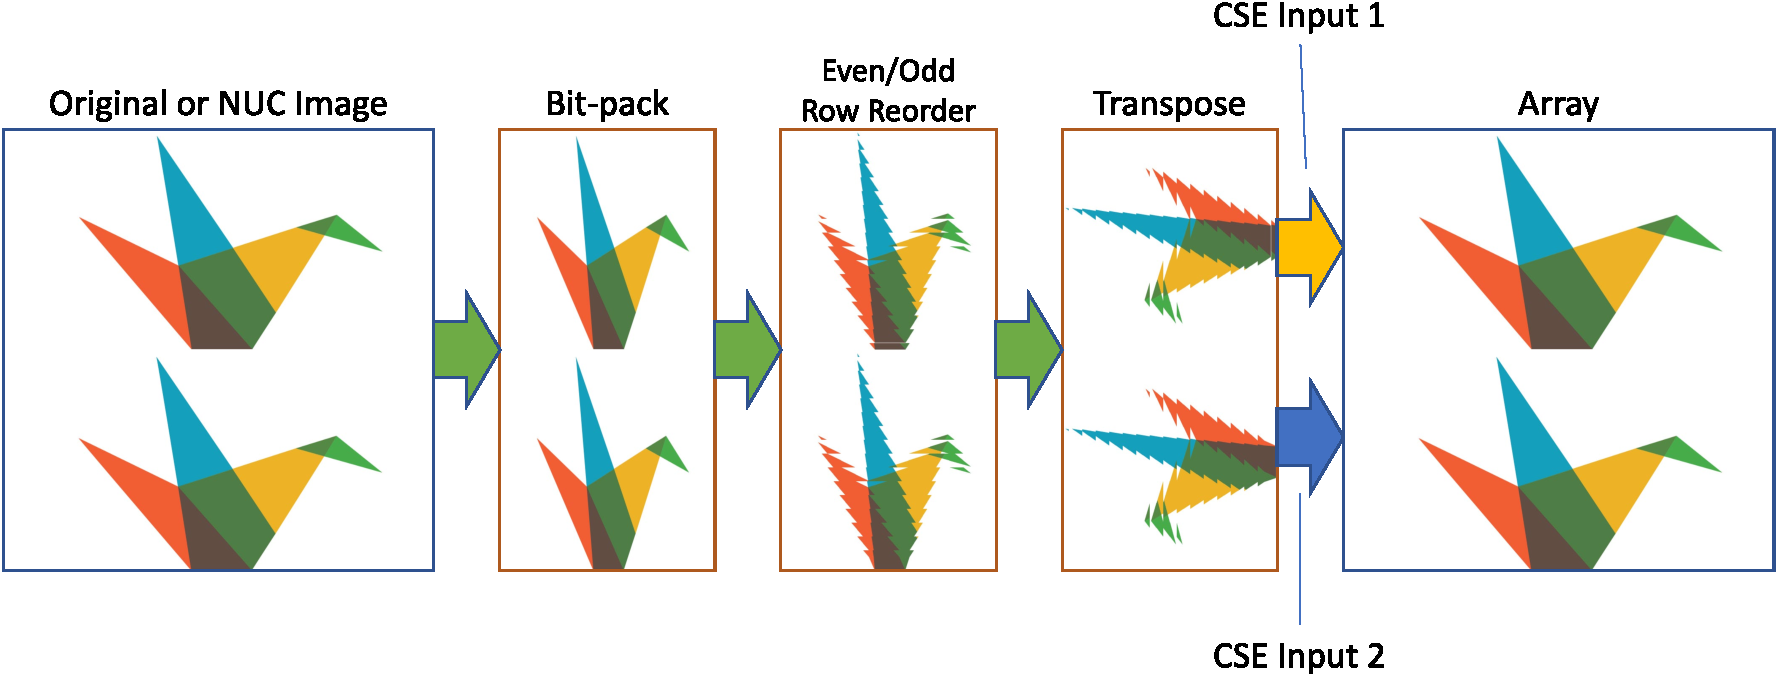
\includegraphics[trim=0 40pt 0 40pt,width=0.90\textwidth]{fig/image_encoding_origami.pdf}
        \caption{Image Encoding: Color Example 3}
        \label{fig:image_encoding_color_example3}
    \end{figure}

    Figures~\ref{fig:image_encoding_ir_example1},~and~\ref{fig:image_encoding_ir_example2} show IR imagery going through the process of reordering. The image shown in Figure~\ref{fig:image_encoding_ir_example1} is commonly used to focus IR cameras and for testing IR array behavior with various shapes and numbers. The image shown in Figure~\ref{fig:image_encoding_ir_example2} is test imagery from one of my labs projects.

    \begin{figure}[H]
        \centering
        %includegraphs[trim=L B R T]
        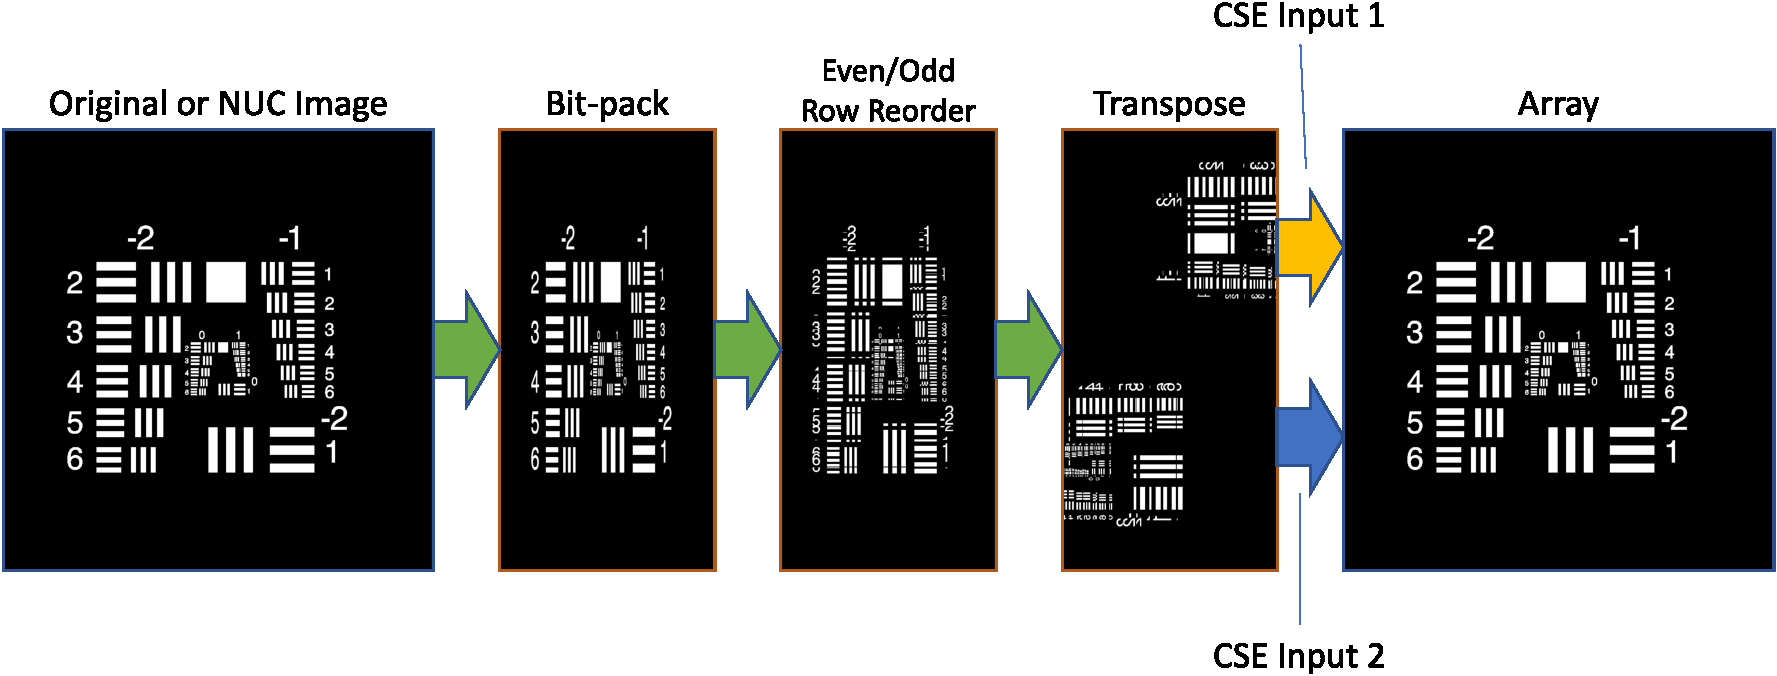
\includegraphics[trim=0 40pt 0 0,width=1.0\textwidth]{fig/image_encoding_ir1.pdf}
        \caption{Image Encoding: IR Example 1}
        \label{fig:image_encoding_ir_example1}
    \end{figure}

    \begin{figure}[H]
        \centering
        %includegraphs[trim=L B R T]
        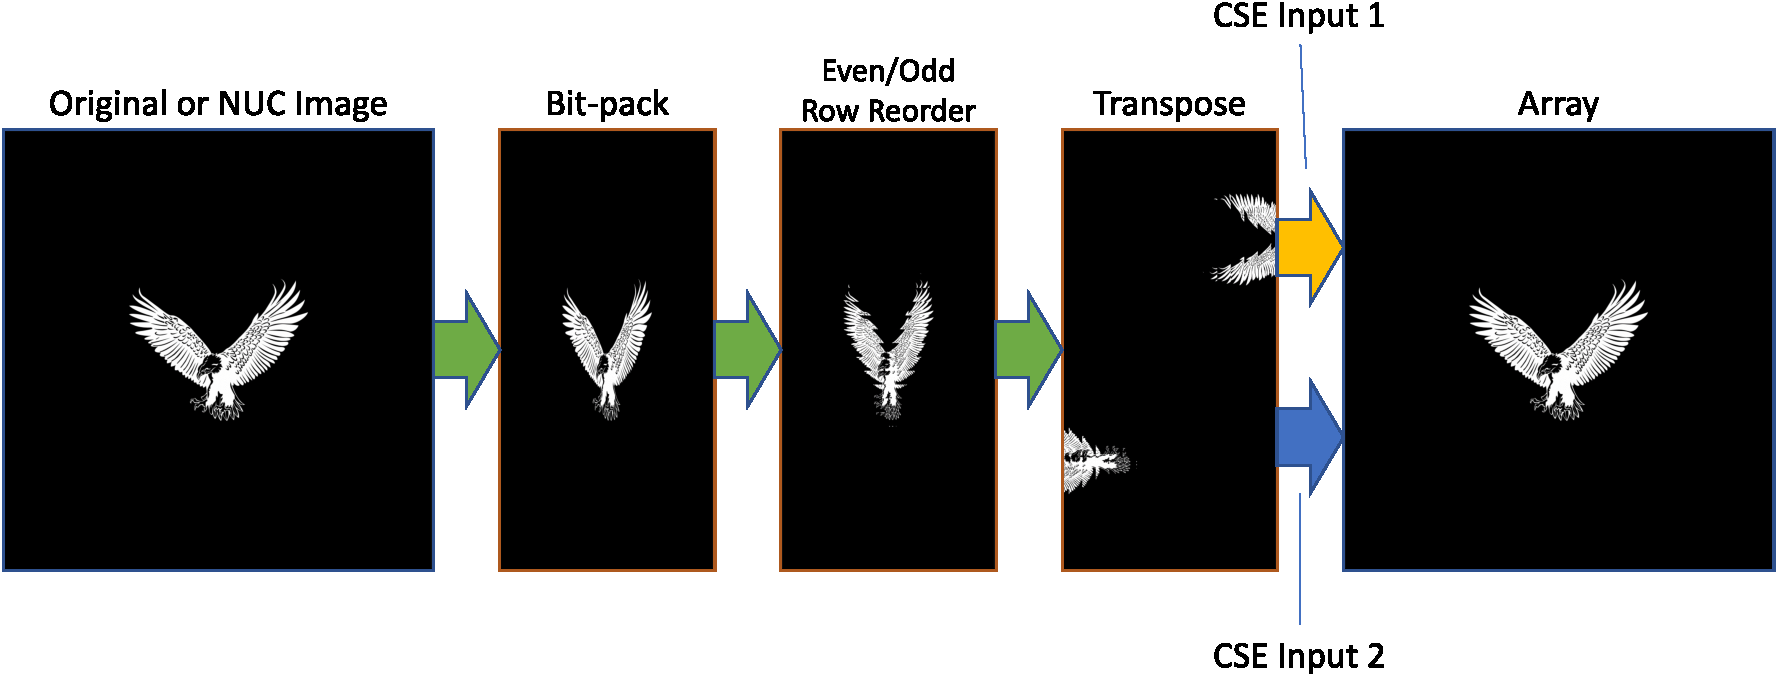
\includegraphics[trim=0 40pt 0 40pt,width=1.0\textwidth]{fig/image_encoding_ir2.pdf}
        \caption{Image Encoding: IR Example 2}
        \label{fig:image_encoding_ir_example2}
    \end{figure}

    While this chapter discussed the internal details of how imagery received within the array is formatted and written to an array, Chapter~\ref{chap:display_protocols} shifts to a discussion of how imagery is sent to an array at the protocol level within an IRLED system while providing details of the limitations and challenges present there.
